\documentclass[a4paper]{article}
\usepackage[T1]{fontenc}
\usepackage[utf8]{inputenc}
\usepackage{CJKutf8}
\usepackage[top=20mm, bottom=20mm, left=20mm, right=20mm]{geometry}
\usepackage{graphicx}
\usepackage{fancyhdr}

\pagestyle{fancy}
\fancyhf{}
\rhead{出席番号:\quad 氏名:}
\lhead{テーマ11 UMLクラス図とオブジェクト図}
\rfoot{\thepage}

\begin{document}
\begin{CJK}{UTF8}{min}

\begin{titlepage}
\begin{center}
\vspace*{30mm}
{\LARGE \textbf{テーマ11 UMLクラス図とオブジェクト図}}
\vspace{20mm}

\begin{table}[h]
\centering
\large
\begin{tabular}{ll}
出席番号: & \\
\hline
氏名: & \\
\hline
\end{tabular}
\end{table}

\vfill

{\large 提出日:2025年9月12日}
\end{center}
\end{titlepage}

\section{IS-A関係の検証}

テーマ10で作成した自作クラスには以下のIS-A関係が存在します:

\begin{itemize}
\item ``Car is a Vehicle''(車は乗り物である)
\item ``ElectricCar is a Car''(電気自動車は車である)
\item ``ElectricCar is a Vehicle''(電気自動車は乗り物である、推移的関係)
\end{itemize}

\newpage

\section{UMLクラス図(概略版)}

\begin{figure}[h]
\centering
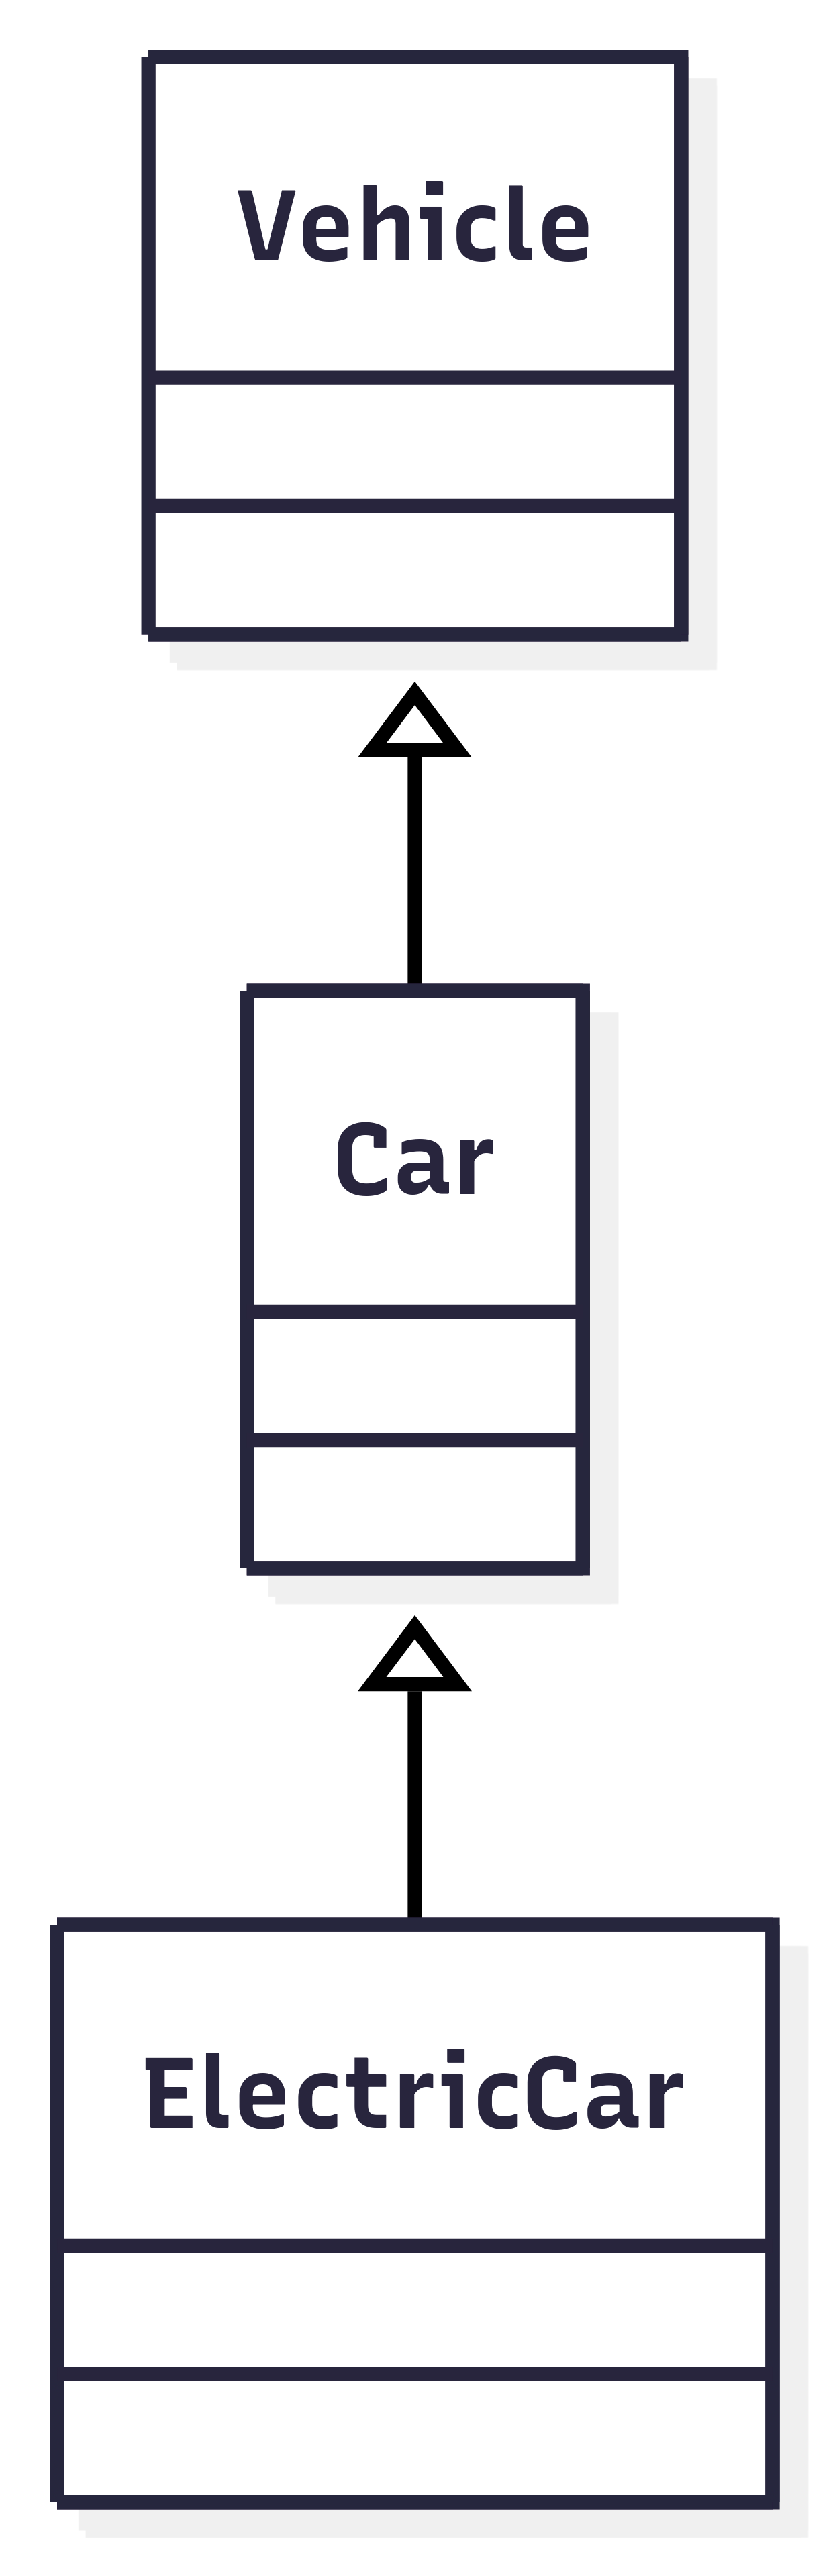
\includegraphics[width=0.1\textwidth]{a.png}
\caption{Vehicle, Car, ElectricCarのUMLクラス図(概略版)}
\end{figure}

\section{UMLクラス図(詳細版)}

\begin{figure}[h]
\centering
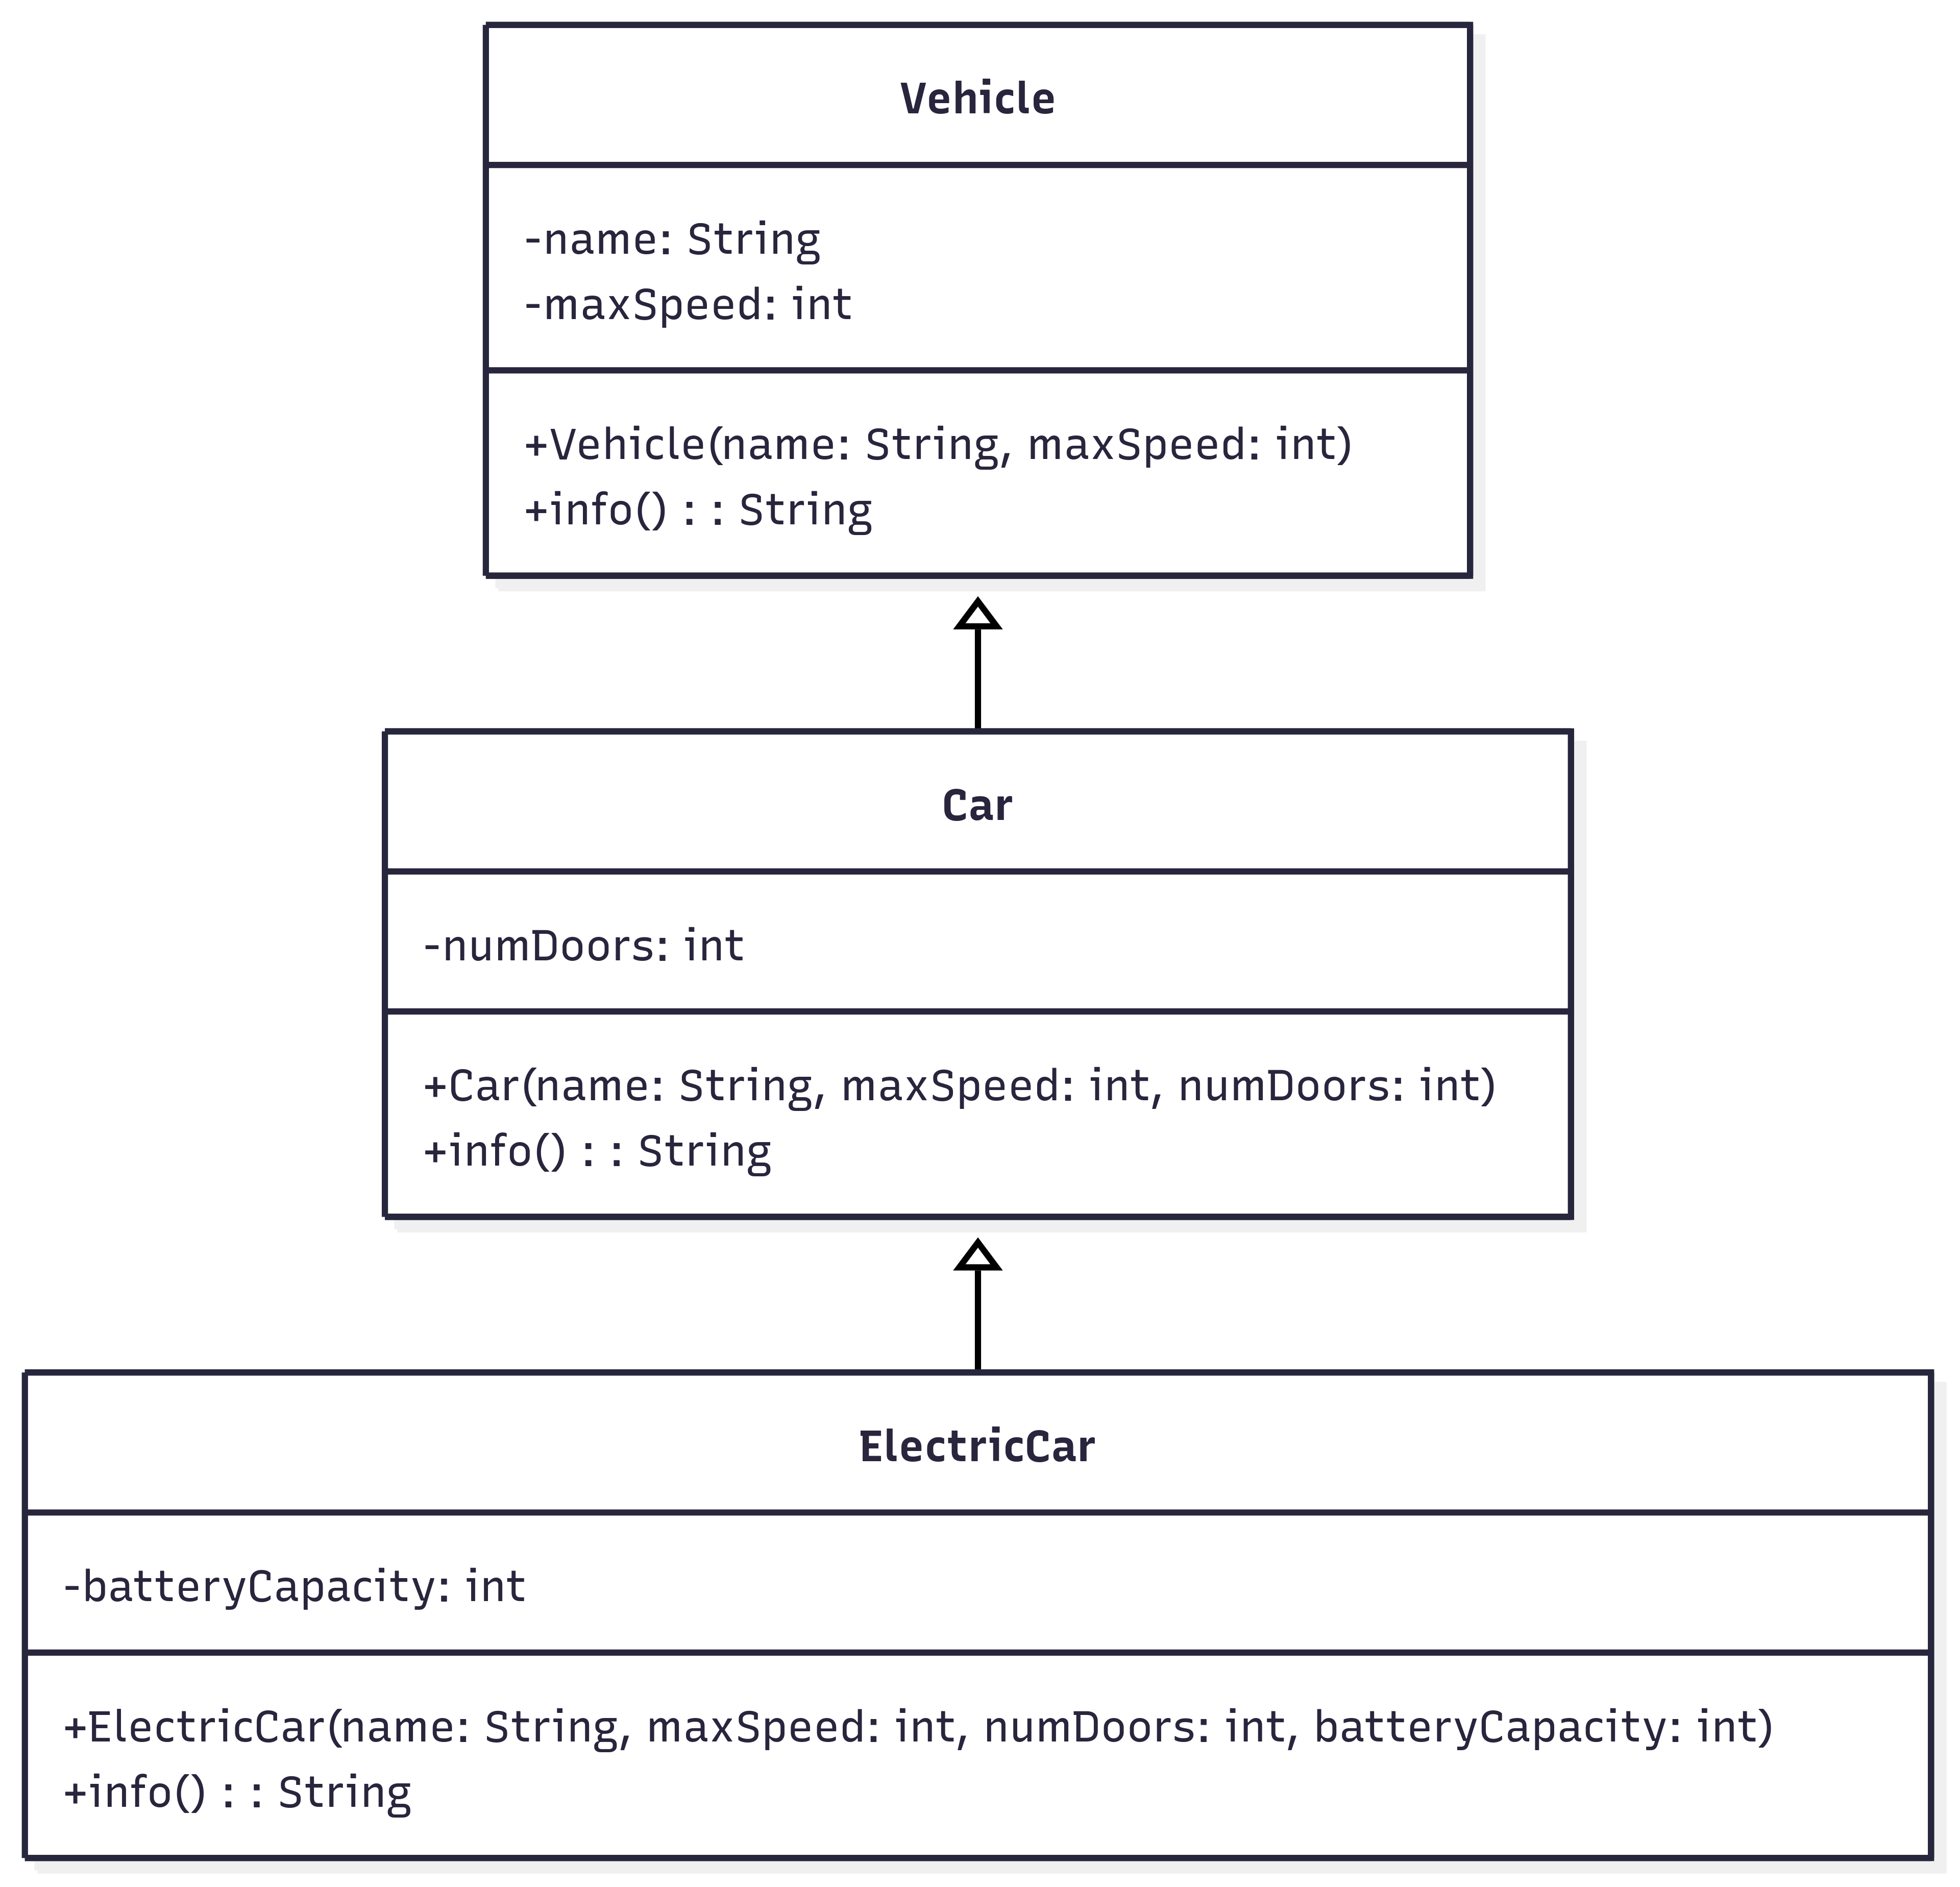
\includegraphics[width=0.7\textwidth]{b.png}
\caption{Vehicle, Car, ElectricCarのUMLクラス図(詳細版)}
\end{figure}

\newpage

\section{テーマ08課題3 UMLオブジェクト図}

\begin{figure}[h]
\centering
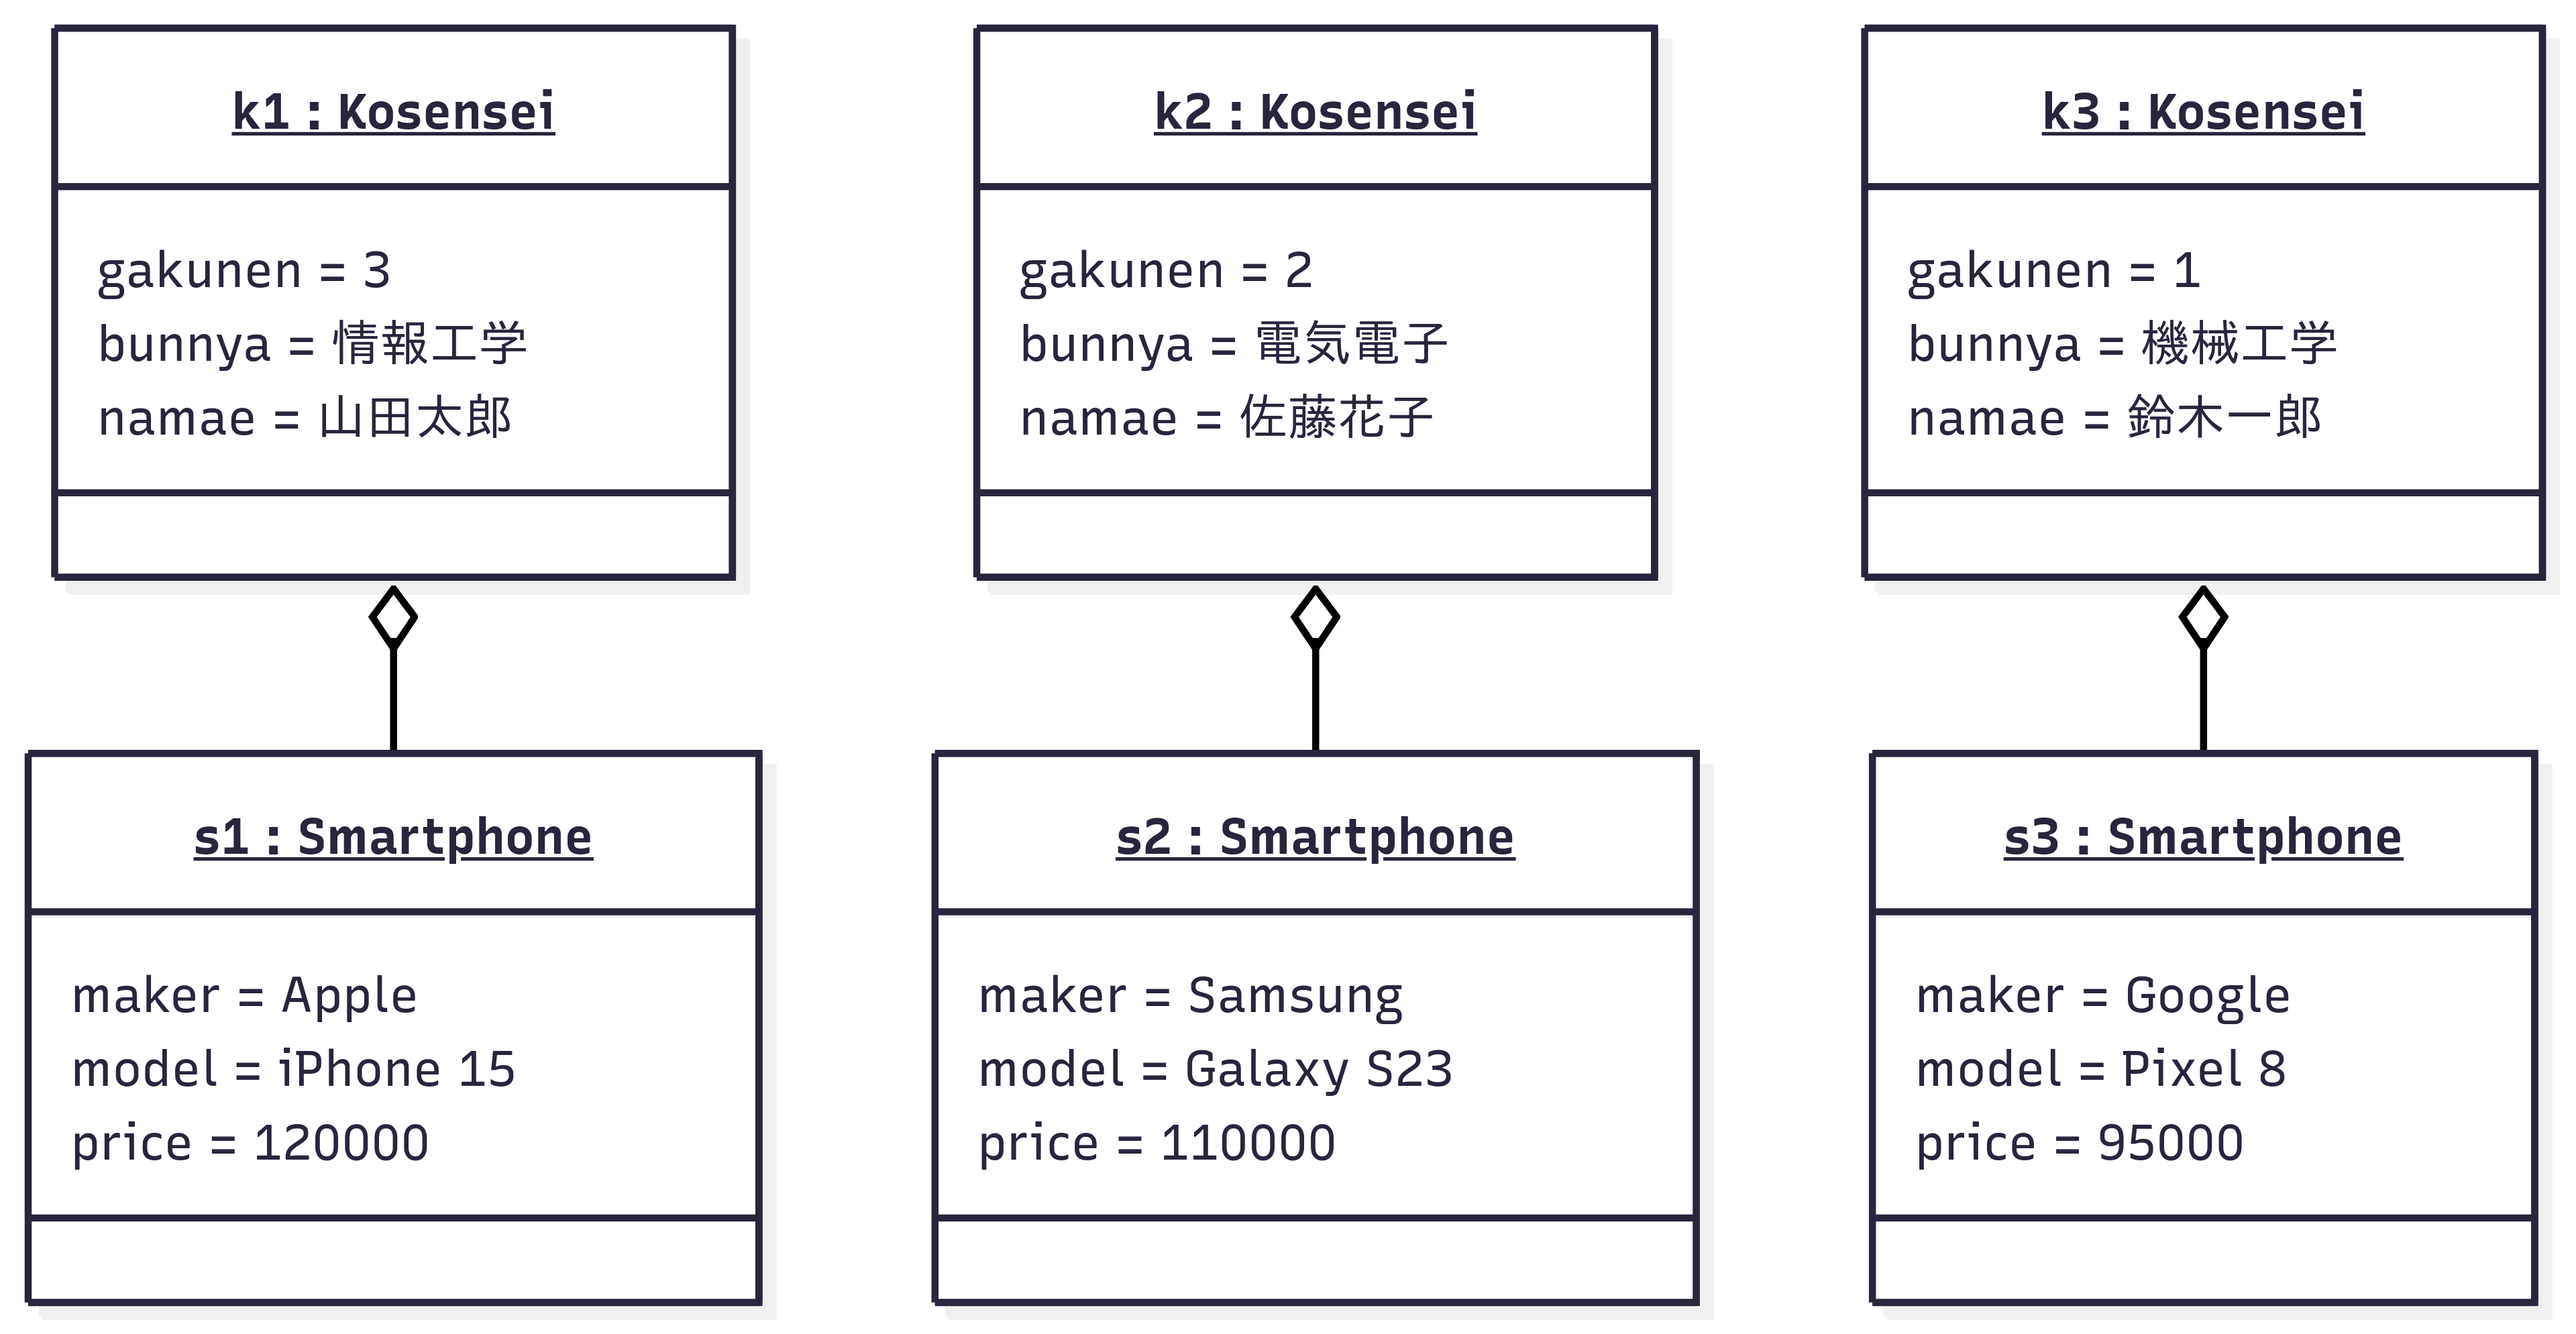
\includegraphics[width=0.7\textwidth]{c.png}
\caption{テーマ08課題3 UMLオブジェクト図}
\end{figure}

\section{テーマ11課題2 UMLオブジェクト図}

\begin{figure}[h]
\centering
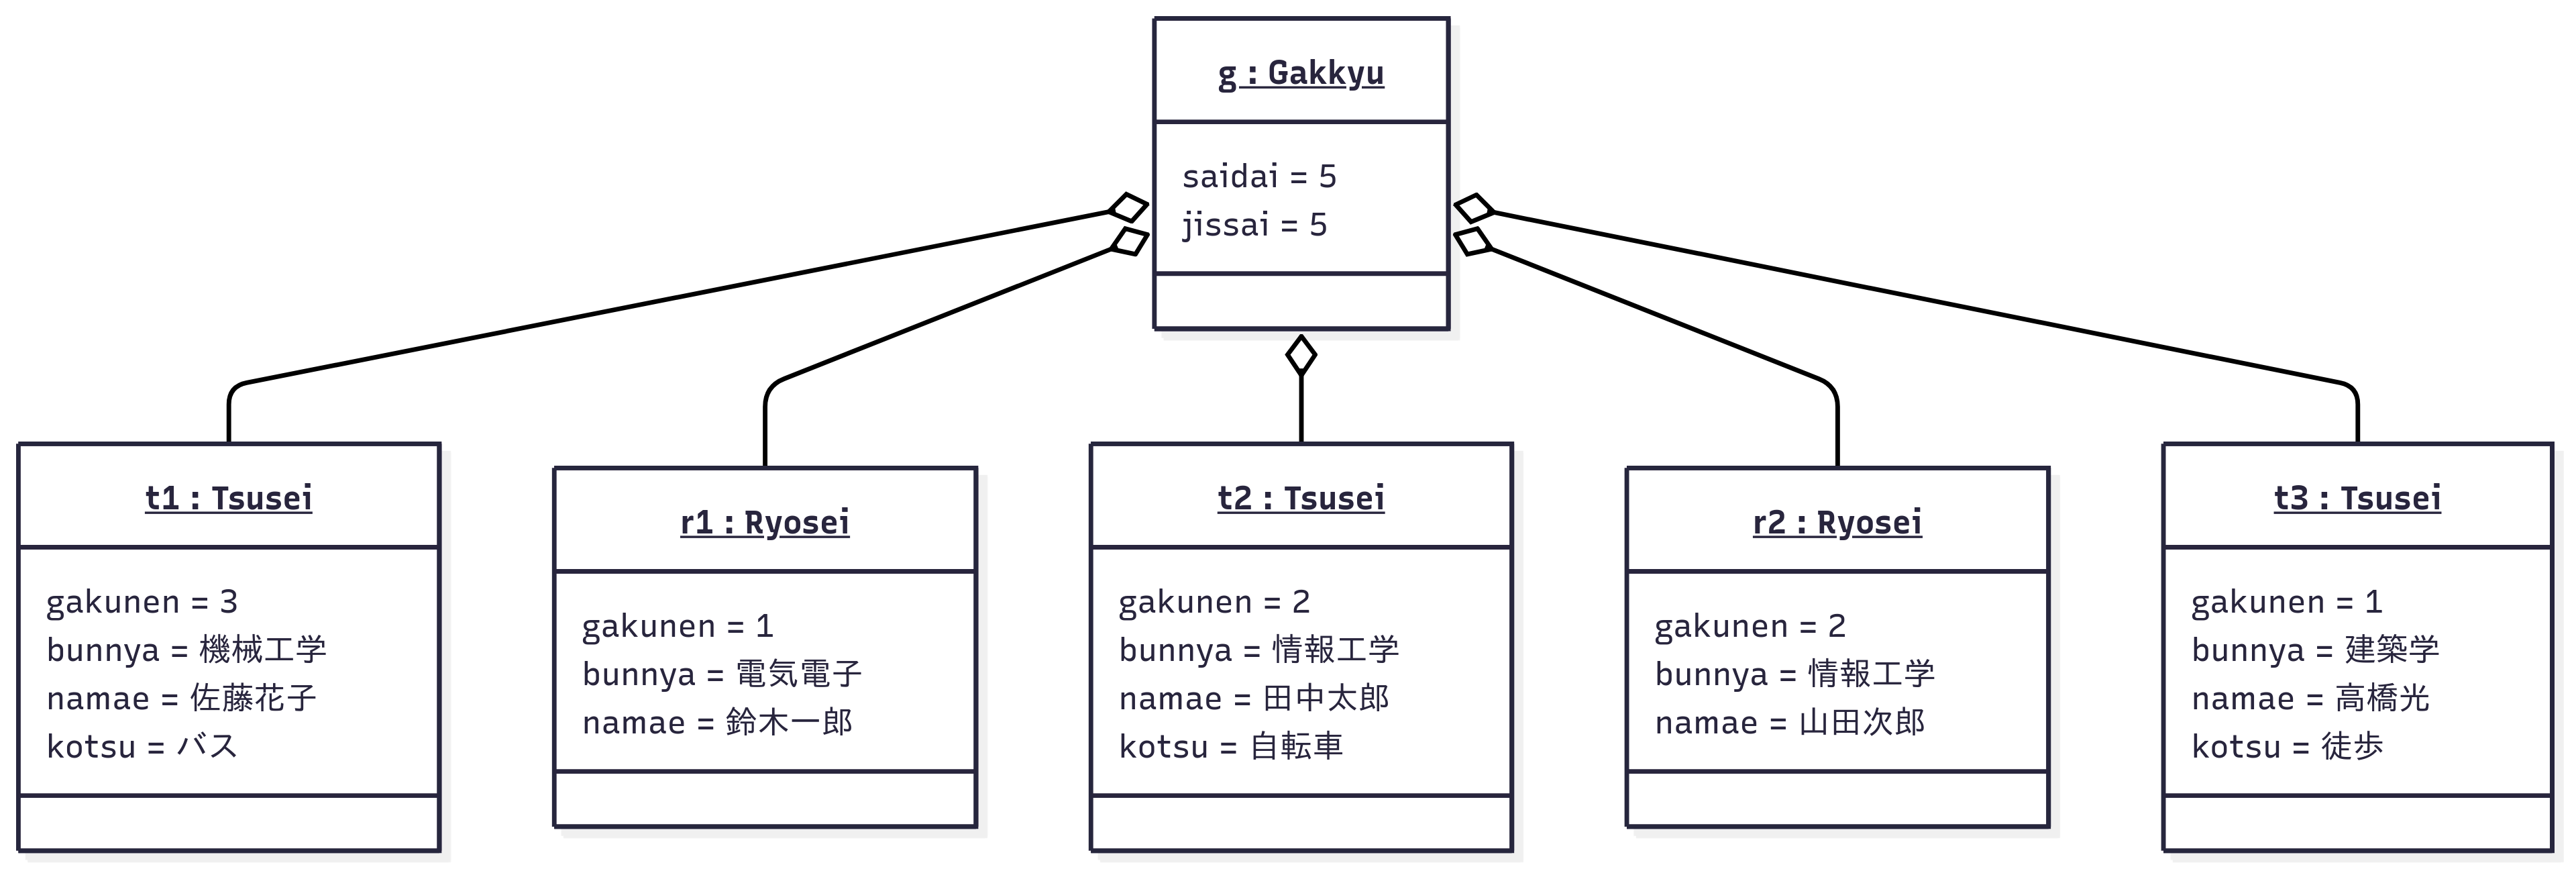
\includegraphics[width=0.7\textwidth]{d.png}
\caption{テーマ11課題2 UMLオブジェクト図}
\end{figure}

\end{CJK}
\end{document}